% !TEX root = comparison.tex
\subsection{Comparing Distributions}

\begin{figure*} [hbtp]
   \centering
   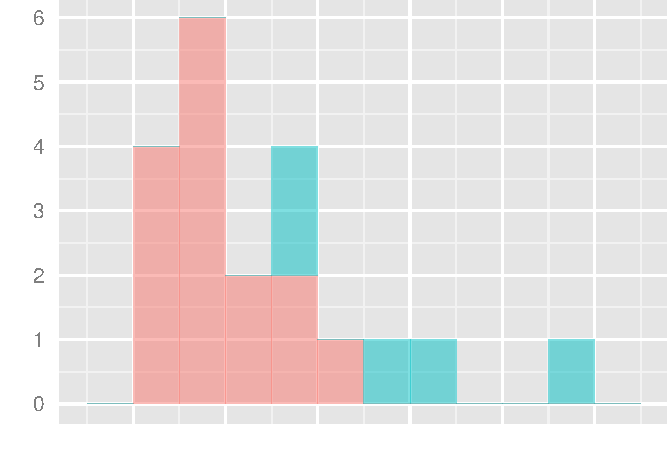
\includegraphics[width=0.245\textwidth]{hist-conc} 
   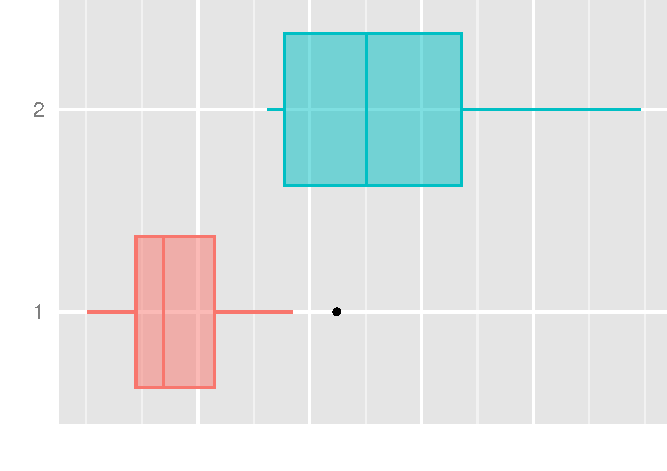
\includegraphics[width=0.245 \textwidth]{boxplot-conc} 
   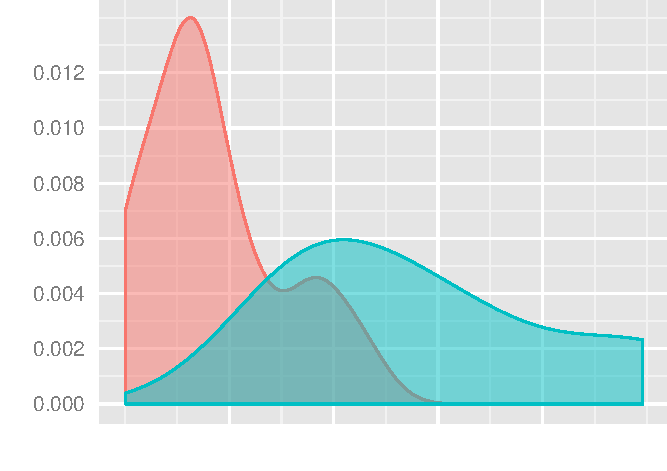
\includegraphics[width=0.245 \textwidth]{density-conc} 
   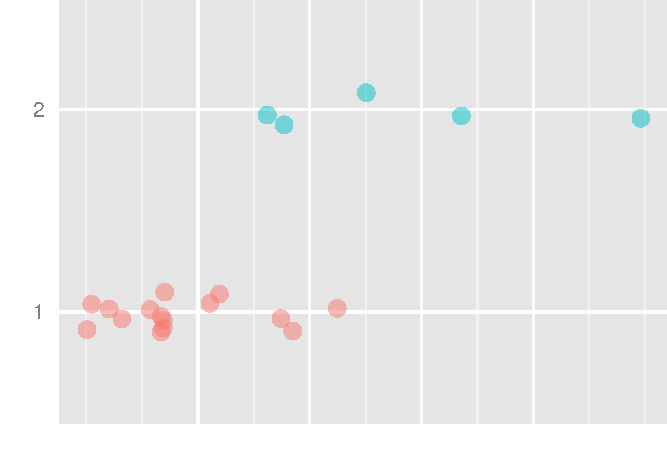
\includegraphics[width=0.245 \textwidth]{dotplot-conc} 
   \caption{Overview of all four competing designs for displaying differences in distributions.}
   \label{fig:expii}
\end{figure*}

\begin{table}[ht]
\begin{center}
\begin{tabular}{rrrrr}
  \hline
 & Estimate & Std. Error & z value & Pr($>$$|$z$|$) \\ 
  \hline
(Intercept) & -2.00 & 0.38 & -5.29 & 0.00 \\ 
  density & -0.29 & 0.53 & -0.55 & 0.58 \\ 
  dotplot & -0.72 & 0.52 & -1.39 & 0.17 \\ 
  histogram & -0.29 & 0.53 & -0.54 & 0.59 \\ 
  d & 1.78 & 0.34 & 5.22 & 0.00 \\ 
  n1 & 0.02 & 0.00 & 9.77 & 0.00 \\ 
  I(n1/n2) & -0.31 & 0.11 & -2.94 & 0.00 \\ 
  density:d & -0.61 & 0.47 & -1.29 & 0.20 \\ 
  dotplot:d & 0.04 & 0.46 & 0.08 & 0.94 \\ 
  histogram:d & -0.29 & 0.48 & -0.60 & 0.55 \\ 
  density:n1 & -0.00 & 0.00 & -0.40 & 0.69 \\ 
  dotplot:n1 & -0.01 & 0.00 & -3.04 & 0.00 \\ 
  histogram:n1 & -0.01 & 0.00 & -2.67 & 0.01 \\ 
  density:I(n1/n2) & 0.09 & 0.15 & 0.59 & 0.55 \\ 
  dotplot:I(n1/n2) & 0.27 & 0.15 & 1.81 & 0.07 \\ 
  histogram:I(n1/n2) & 0.09 & 0.15 & 0.62 & 0.53 \\ 
   \hline
\end{tabular}
\end{center}
\caption{correctness}
\end{table}

\begin{table}[ht]
\begin{center}
\begin{tabular}{rrrrr}
  \hline
 & Estimate & Std..Error & t.value & pval \\ 
  \hline
(Intercept) & 3.85 & 0.09 & 42.21 & 0.00 \\ 
  density & 0.01 & 0.12 & 0.07 & 0.94 \\ 
  dotplot & 0.03 & 0.12 & 0.26 & 0.80 \\ 
  histogram & 0.23 & 0.12 & 1.97 & 0.05 \\ 
  d & -0.23 & 0.08 & -3.02 & 0.00 \\ 
  n1 & 0.00 & 0.00 & 1.74 & 0.08 \\ 
  I(n1/n2) & -0.04 & 0.02 & -1.48 & 0.14 \\ 
  density:d & 0.11 & 0.11 & 1.02 & 0.31 \\ 
  dotplot:d & 0.20 & 0.11 & 1.86 & 0.06 \\ 
  histogram:d & -0.01 & 0.11 & -0.09 & 0.93 \\ 
  density:n1 & -0.00 & 0.00 & -2.15 & 0.03 \\ 
  dotplot:n1 & -0.00 & 0.00 & -2.87 & 0.00 \\ 
  histogram:n1 & -0.00 & 0.00 & -0.93 & 0.35 \\ 
  density:I(n1/n2) & 0.04 & 0.03 & 1.18 & 0.24 \\ 
  dotplot:I(n1/n2) & 0.02 & 0.03 & 0.65 & 0.52 \\ 
  histogram:I(n1/n2) & 0.00 & 0.04 & 0.04 & 0.97 \\ 
   \hline
\end{tabular}
\end{center}
\caption{log time taken}

\end{table}



